%% Time-stamp: <2019-01-22 14:47:04 (marc)>
\documentclass[xcolor=x11names,compress, mathserif]{beamer}
\newcommand\hmmax{0}
\newcommand\bmmax{0}

\usepackage{../includes/MarkMathCmds}

\newcommand{\hackspace}{\hspace{4.2mm}}
\newcommand{\showstudent}[1]{}



% talk/author information
\newcommand{\authorname}{Mark van der Wilk}
\newcommand{\authoremail}{m.vdwilk@imperial.ac.uk}
\newcommand{\authoraffiliation}{
 Department of Computing\\Imperial
  College London}
\newcommand{\authortwitter}{markvanderwilk}
\newcommand{\slidesettitle}{\imperialBlue{Sequential Decisions}}
\newcommand{\footertitle}{Sequential Decisions}
\newcommand{\location}{Imperial College London}
\newcommand{\talkDate}{{February 13, 2023}}


\usepackage{tikz}
\tikzset{
  treenode/.style = {shape=rectangle, rounded corners,
                     draw, align=center,
                     top color=white, bottom color=blue!20},
  root/.style     = {treenode, font=\Large, bottom color=red!30},
  env/.style      = {treenode, font=\ttfamily\normalsize},
  dummy/.style    = {circle,draw}
}




\date{\imperialGray{\talkDate}}




% load defaults
\input{../includes/header.tex}
\input{../includes/titlepage.tex}



\begin{frame}{Sequential Decision Making}
\begin{itemize}
\item Last time: Principle for taking an action based on beliefs. \pause
\item This time: How do we plan for decisions made after each other? \pause
\item Key idea: At each point, apply MEU, given all the knowledge you have at that point \pause
\item Consequence: After making an earlier decision, you can \emph{learn}. This information has value. \pause
\item This is key reason why things become complicated, but principle is no more complex!
\end{itemize}
\end{frame}


\begin{frame}[allowframebreaks]{Example: Commuting}
Paula has an exam at 9am today, and it is 8:35am. She will not be admitted if she is late, so her loss function is
\begin{align}
L(t, a) = \begin{cases}
0 & \text{if } t \leq 25 \text{ min} \\
100 & \text{if } t > 25 \text{ min}
\end{cases} \,.
\end{align}

Paula decides to take a taxi. The taxi driver knows of routes A and B. Route A can either be clear and fast ($Q=0$) or jammed and slow ($Q=1$). The time for route B follows a Gaussian.
\begin{gather}
% p(t_\text{A}) &= \begin{cases}
% 10 \text{ min} & \text{with probability } 0.5 \\
% 50 \text{ min} & \text{with probability } 0.5
% \end{cases} \,, \\
t_\text{A} = \begin{cases}
10 \text{ min} & \text{if } Q = 0 \\
50 \text{ min} & \text{if } Q = 1
\end{cases} \,, \qquad
P(Q) = \begin{cases}
0.5 & \text{for } Q = 0 \\
0.5 & \text{for } Q = 1
\end{cases} \,, \\
p(t_\text{B}) = \NormDist{t_\text{B}; 25, 5^2} \,.
\end{gather}


\vspace{1.0cm}
The driver suggests the following strategy:
\begin{itemize}
\item Drive the first 2.5 minutes of route A to see whether it is clear (i.e.~to observe $Q$).
\item At that point, decide whether to keep going with route A, or to drive back 2.5 minutes and take route B.
\end{itemize}

\vspace{0.5cm}

Question: Should Paula:
\begin{itemize}
\item Ask the driver to take route A?
\item Ask the driver to take route B?
\item Ask the driver to continue with his strategy?
\end{itemize}
\end{frame}


\begin{frame}{Decision Trees}
\begin{itemize}
\item Arrange sequence of observations and decisions into a \emph{tree}
\item Helps us to compute utility based on decisions
\item Helps us to find sequence of optimal decisions
\vspace{0.5cm}
\item Rectangle: Decision nodes.
\item Circle: Observation of a random variable.
\item Leaf nodes: Outcome of utility.
\item Nodes are functions of the outcome of parent RVs.
\end{itemize}
\end{frame}


\begin{frame}{Finding optimal decisions}
Simple process:
\begin{itemize}
\item Start at leaf nodes and move towards root.
\item RV nodes: Calculate expectation over utility values coming in.
\item Decision nodes: Choose action corresponding to child with maximum utility. Pass on this utility.
\end{itemize}
\end{frame}



\begin{frame}{Example: Commuting}
\scalebox{0.6}{
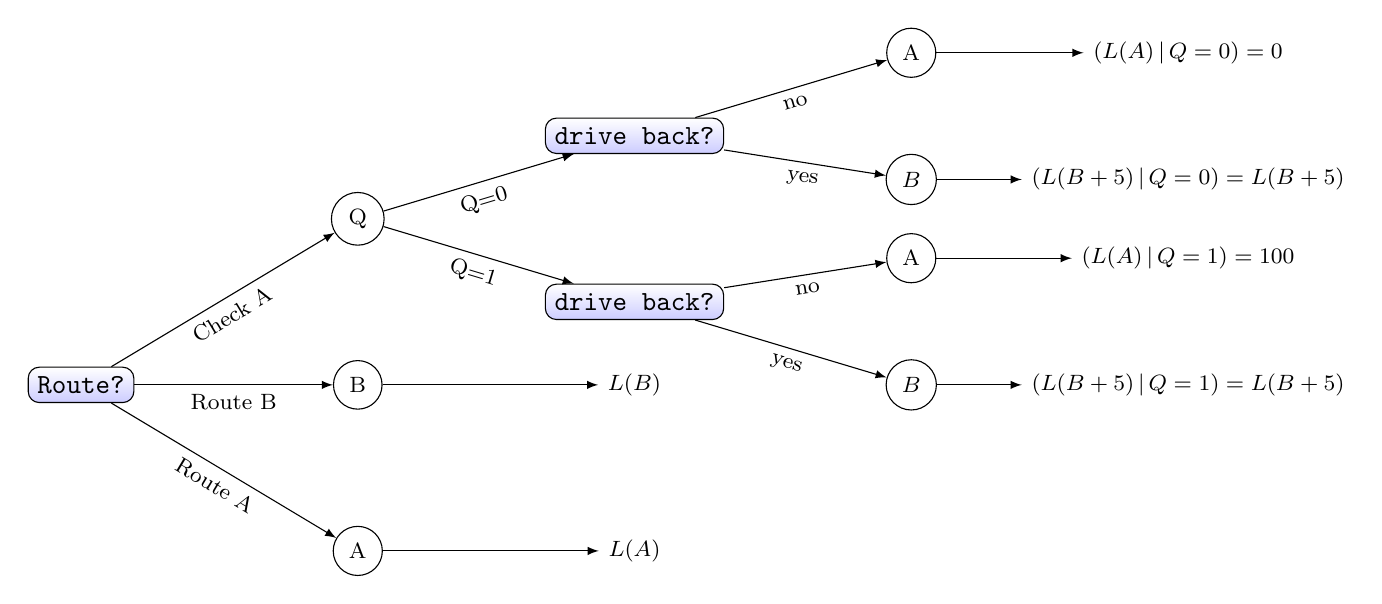
\begin{tikzpicture}
  [
    grow                    = right,
    sibling distance        = 6em,
    level distance          = 10em,
    edge from parent/.style = {draw, -latex},
    every node/.style       = {font=\footnotesize},
    sloped
  ]
 \node [env] {Route?}
    child { node [dummy] {A}
      child { node [] {$L(A)$}
        edge from parent node [below] {} }
      edge from parent node [below] {Route A} }
    child { node [dummy] {B}
      child { node [] {$L(B)$}
        edge from parent node [below] {} }
      edge from parent node [below] {Route B} }
    child { node [dummy] {Q}
      child { node [env] {drive back?}
        child { node [dummy] {$B$}
          child { node [] {$(L(B + 5) \,|\, Q = 1) = L(B + 5)$}
            edge from parent node [below] {} }
          edge from parent node [below] {yes} }
        child { node [dummy,yshift=-0.5cm] {A}
          child { node [] {$(L(A) \,|\, Q = 1) = 100$}
            edge from parent node [below] {} }
          edge from parent node [below] {no} }
        edge from parent node [below] {Q=1} }
      child { node [env] {drive back?}
        child { node [dummy,yshift=0.5cm] {$B$}
          child { node [] {$(L(B + 5) \,|\, Q = 0) = L(B+5)$}
            edge from parent node [below] {} }
          edge from parent node [below] {yes} }
        child { node [dummy] {A}
          child { node [] {$(L(A) \,|\, Q = 0) = 0$}
            edge from parent node [below] {} }
          edge from parent node [below] {no} }
        edge from parent node [below] {Q=0} }
      edge from parent node [below] {Check A} }
;
\end{tikzpicture}}

\begin{itemize}
\item We can split up outcomes of RVs explicitly
\item This allows us to find explicit numerical values at all points.
\item Note: $(L(B + 5) \,|\, Q = 0) = L(B+5)$, since $B \ci Q$.
\end{itemize}
{\tiny Board: solution.}
\end{frame}




\begin{frame}{Example: Commuting}
\scalebox{0.6}{
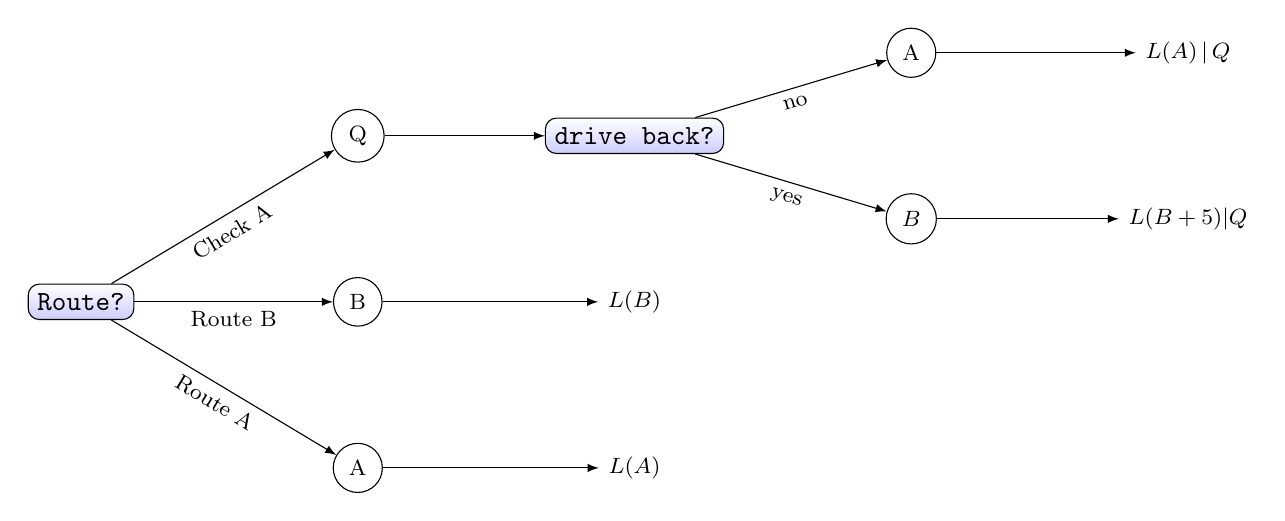
\begin{tikzpicture}
  [
    grow                    = right,
    sibling distance        = 6em,
    level distance          = 10em,
    edge from parent/.style = {draw, -latex},
    every node/.style       = {font=\footnotesize},
    sloped
  ]
 \node [env] {Route?}
    child { node [dummy] {A}
      child { node [] {$L(A)$}
        edge from parent node [below] {} }
      edge from parent node [below] {Route A} }
    child { node [dummy] {B}
      child { node [] {$L(B)$}
        edge from parent node [below] {} }
      edge from parent node [below] {Route B} }
    child { node [dummy] {Q}
      child { node [env] {drive back?}
        child { node [dummy] {$B$}
          child { node [] {$L(B + 5)|Q$}
            edge from parent node [below] {} }
          edge from parent node [below] {yes} }
        child { node [dummy] {A}
          child { node [] {$L(A) \,|\, Q$}
            edge from parent node [below] {} }
          edge from parent node [below] {no} }
        edge from parent node [below] {} }
      edge from parent node [below] {Check A} }
;
\end{tikzpicture}}

\begin{itemize}
\item Can make graph smaller by not writing out all outcomes of RVs.
\item Decisions become \textit{functions} of parent outcomes.
\end{itemize}
{\tiny Board: solution}
\end{frame}

\begin{frame}{Exploration-Exploitation Trade-Off}
\begin{itemize}
\item We saw that ``Check A'' was the best option.
\item Spending effort to gather information, can help us to make better decisions later.
\item Uncertainty determines how much exploration can gain.
\item (Would exploration be worth it if $P(Q=1) = 0.99$?)
\item \arrow Exploration-exploitation trade-off.
\end{itemize}
\end{frame}


\begin{frame}{Conclusion}
\begin{itemize}
\item Sequential decision making is the same as earlier.
\item Can deal with complexity using decision trees.
\item Exploration-exploitation trade-off.
\end{itemize}

\vspace{0.5cm}

Recommended reference: MacKay \cite{itila} chapter 36. \\
Further reading: Russell \cite{russell} chapter 17. \\
There's a whole theory of MDPs out there!
\end{frame}





%%%%%%%%%%%%%%%%%%%%%%%%%%%%%%%%%%%%%%%%%
% REFERENCES
%%%%%%%%%%%%%%%%%%%%%%%%%%%%%%%%%%%%%%%%%
\begin{frame}[t,allowframebreaks]
\frametitle{References}
\linespread{1.0}
\tiny
\bibliographystyle{abbrv}
\bibliography{../includes/pi-literature.bib}
\end{frame}



\end{document}
%%% Local Variables: 
%%% mode: latex
%%% TeX-master: t
%%% End: 
